\section{Mis primeros shader de juguete}
\begin{frame}{Repositorio}
Todo lo necesario para este taller esta en este repositorio: 
\begin{block}{}
\url{https://github.com/nemediano/tallerShadertoy}.
\end{block}
\begin{itemize}
    \item Ésta presentación, también esta en el mismo repositorio. Así puedes seguir los links.
    \item Para cada ejercicio, hay dos versiones de código fuente.
    \begin{enumerate}
        \item El código mínimo para empezar el ejercicio
        \item Una posible solución al ejercicio 
    \end{enumerate}
\end{itemize}

\end{frame}

\begin{frame}{Últimos detalles}
En shadertoy, la ejecución inicia y termina con la función:

\mintinline{glsl}{void mainImage(out vec4 fragColor, in vec2 fragCoord)}.

\begin{itemize}
    \item Por cada fragment recibes de parámetro: \mintinline{glsl}{fragCoord}, con la posición del fragment en el \emph{render target}.
    \item La salida: \mintinline{glsl}{fragColor}, es un output parameter. Un vector de dimensión 4 que debe contener el color final del fragment.
    \begin{itemize}
        \item La salida $\mathbf{x} \in \mathbb{R}^{4}$ debe tener $ x_i \in [0, 1]$.
        \item El último componente $x_4$ (ó bien $w$), representa el componente alpha, que en Shadertoy debe ser 1.
    \end{itemize}
\end{itemize}
\end{frame}

\begin{frame}{Ejercicio: Bandera a cuadros}
\url{https://github.com/nemediano/tallerShadertoy/tree/main/codigo/Ejercicio1}
\begin{columns}
\column[t]{0.5\textwidth}
     \begin{itemize}
         \item Tratar de escribir un shader que genere una bandera a cuadros (o tablero de ajedrez si lo prefieres)
         \item Puedes empezar con el código de default de shader toy.
         \item Recuerda las funciones trigonométricas
     \end{itemize}
\column[t]{0.5\textwidth}
        \begin{figure}[htb]
            \centering
            
\includegraphics[width=0.6\textwidth]{img/Ejer1}
        \end{figure}
\end{columns}
\end{frame}


\subsection{Funciones de distancia}

\begin{frame}{Sistema de coordenadas}
\begin{columns}
\column[t]{0.5\textwidth}
    \begin{itemize}
         \item Al principio, las coordenadas del fragment están en el espacio del imagen del render target. Miden pixeles.
         \item Cuando dividimos entre la resolución del render target, están en coordenadas de textura ($uv$-mapping). $u,v \in [ 0,1 ]$
     \end{itemize}
\column[t]{0.5\textwidth}
\begin{figure}[htp]
 \centering
 \begin{subfigure}[b]{0.45\textwidth}
   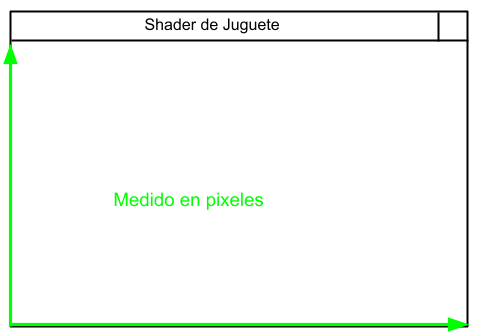
\includegraphics[width=\textwidth]{img/FrameOfreference}
   \caption{Espacio de imagen}
 \end{subfigure}
\\
 \begin{subfigure}[b]{0.45\textwidth}
   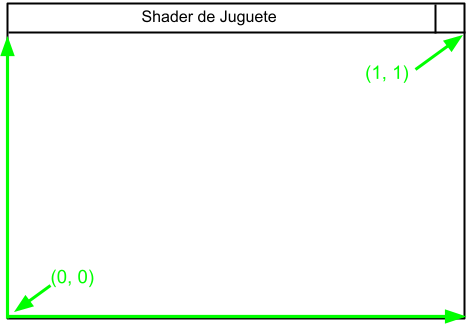
\includegraphics[width=\textwidth]{img/FoRUVSpace}
   \caption{$uv$ space}
 \end{subfigure}
\end{figure}
\end{columns}
\end{frame}

\begin{frame}{Sistema de coordenadas II}
\begin{columns}
\column[t]{0.5\textwidth}
    \begin{itemize}
        \item Cuando restamos 0.5 y multiplicamos por dos. Están en coordenadas normalizadas. $x,y \in [-1, 1]$.
        \item Cuando corregimos con el \emph{aspect ratio} de la pantalla, están en coordenadas de la escena. El origen esta en el centro, el eje mas restrictivo esta en $[-1, 1]$ y el otro es proporcional.
     \end{itemize}
\column[t]{0.5\textwidth}
\begin{figure}[htp]
 \centering
 \begin{subfigure}[b]{0.45\textwidth}
   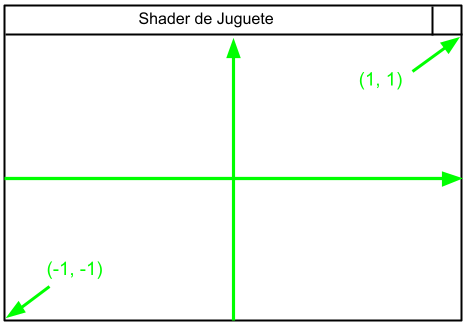
\includegraphics[width=\textwidth]{img/FoRNormalized}
   \caption{Normalize coordinates}
 \end{subfigure}
\\
 \begin{subfigure}[b]{0.45\textwidth}
   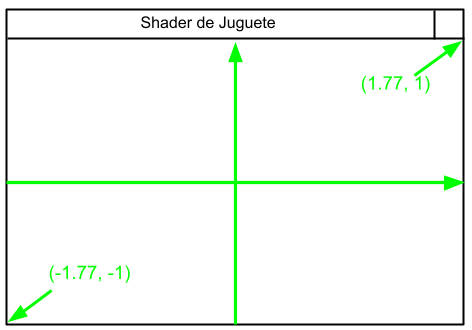
\includegraphics[width=\textwidth]{img/FoRCorrected}
   \caption{World Coordinates}
 \end{subfigure}
\end{figure}
\end{columns}
\end{frame}

\begin{frame}[fragile]{Función de transformación}
\begin{listing}
\begin{minted}{glsl}
vec3 getWorldCoordinates(vec2 fragCoord, vec3 iResolution) {

    float aspectRatio = iResolution.x / iResolution.y;

    vec2 scaleFactor =
        iResolution.x > iResolution.y ? vec2(aspectRatio, 1.0) : vec2(1.0, 1.0 / aspectRatio);

    vec2 world = scaleFactor * (2.0 * (fragCoord/iResolution.xy) - vec2(1.0));

    return vec3(world, 1.0);
}
\end{minted}
\end{listing}
Después veremos por que esta función, de hecho regresa un vector en $\mathbb{R}^3$, cuyo tercer componente es 1.
\end{frame}


\begin{frame}{Función de distancia con signo}

\begin{itemize}
    \item En Inglés mejor conocida como: \emph{signed distance field} (sdf).
    \item Hay una \href{https://en.wikipedia.org/wiki/Signed_distance_function}{definición formal}. Pero intuitivamente:
    \begin{itemize}
        \item Si tienes una curva cerrada $c$ en $\mathbb{R}^n$, cuya frontera es $\delta$.
        \item Entonces la $sdf(c)$ es una función continua $sdf: \mathbb{R}^n \rightarrow \mathbb{R}$, tal que es positiva en el exterior de $f$, negativa en el interior de $f$ y cero en $\delta$.
    \end{itemize}
\end{itemize}
\begin{columns}
\column[t]{0.4\textwidth}
     \begin{itemize}
         \item Para el circulo $x^2 + y^2 = 1$
         \item Una posible sdf es: $x^2 + y^2 - 1$
     \end{itemize}
\column[t]{0.6\textwidth}
        \begin{figure}[htb]
            \centering
            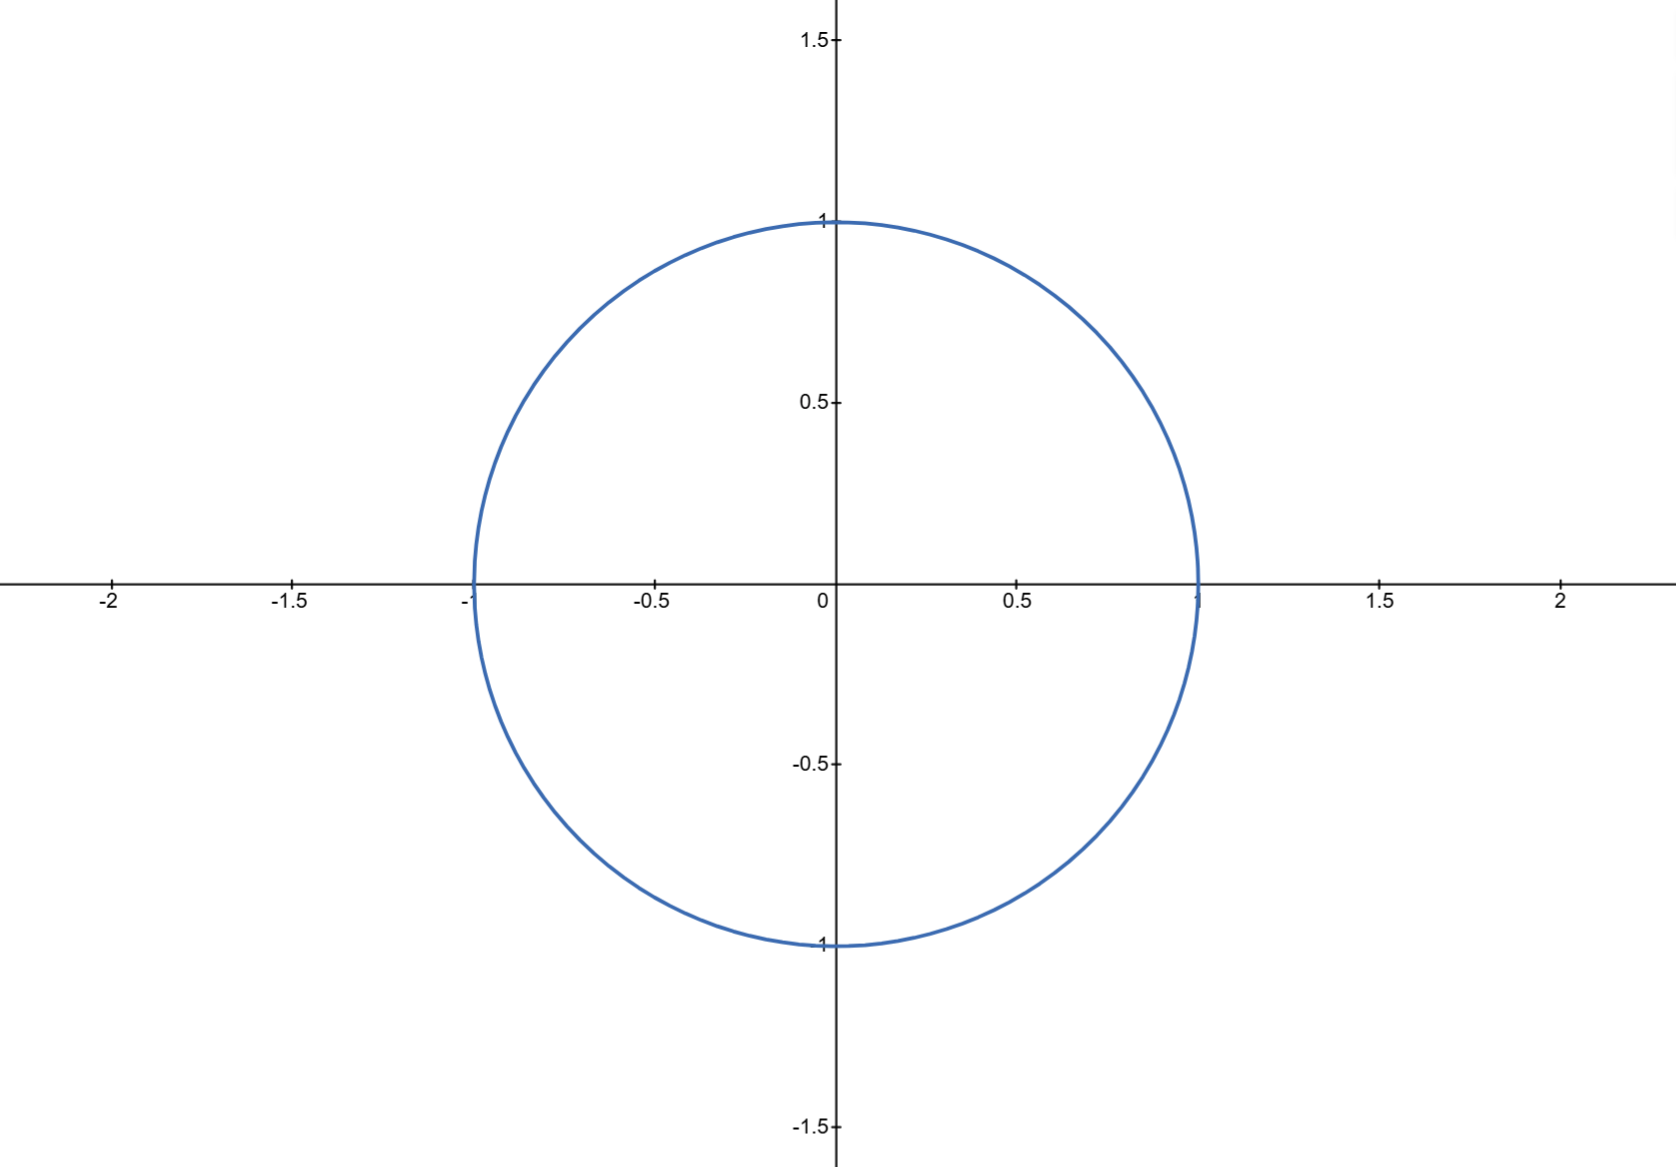
\includegraphics[width=0.6\textwidth]{img/unitCircle.png}
        \end{figure}
\end{columns}
\end{frame}

\begin{frame}{Ejercicio: Un cuadrado detrás de un circulo}
\url{https://github.com/nemediano/tallerShadertoy/tree/main/codigo/Ejercicio2}
\begin{columns}
\column[t]{0.5\textwidth}
     \begin{itemize}
         \item Abstraer el código en funciones
         \item Tener una función que cambia las coordenadas
         \item Tener una función para el fondo
         \item Puedes utilizar la guía de colores
     \end{itemize}
\column[t]{0.5\textwidth}
        \begin{figure}[htb]
            \centering
            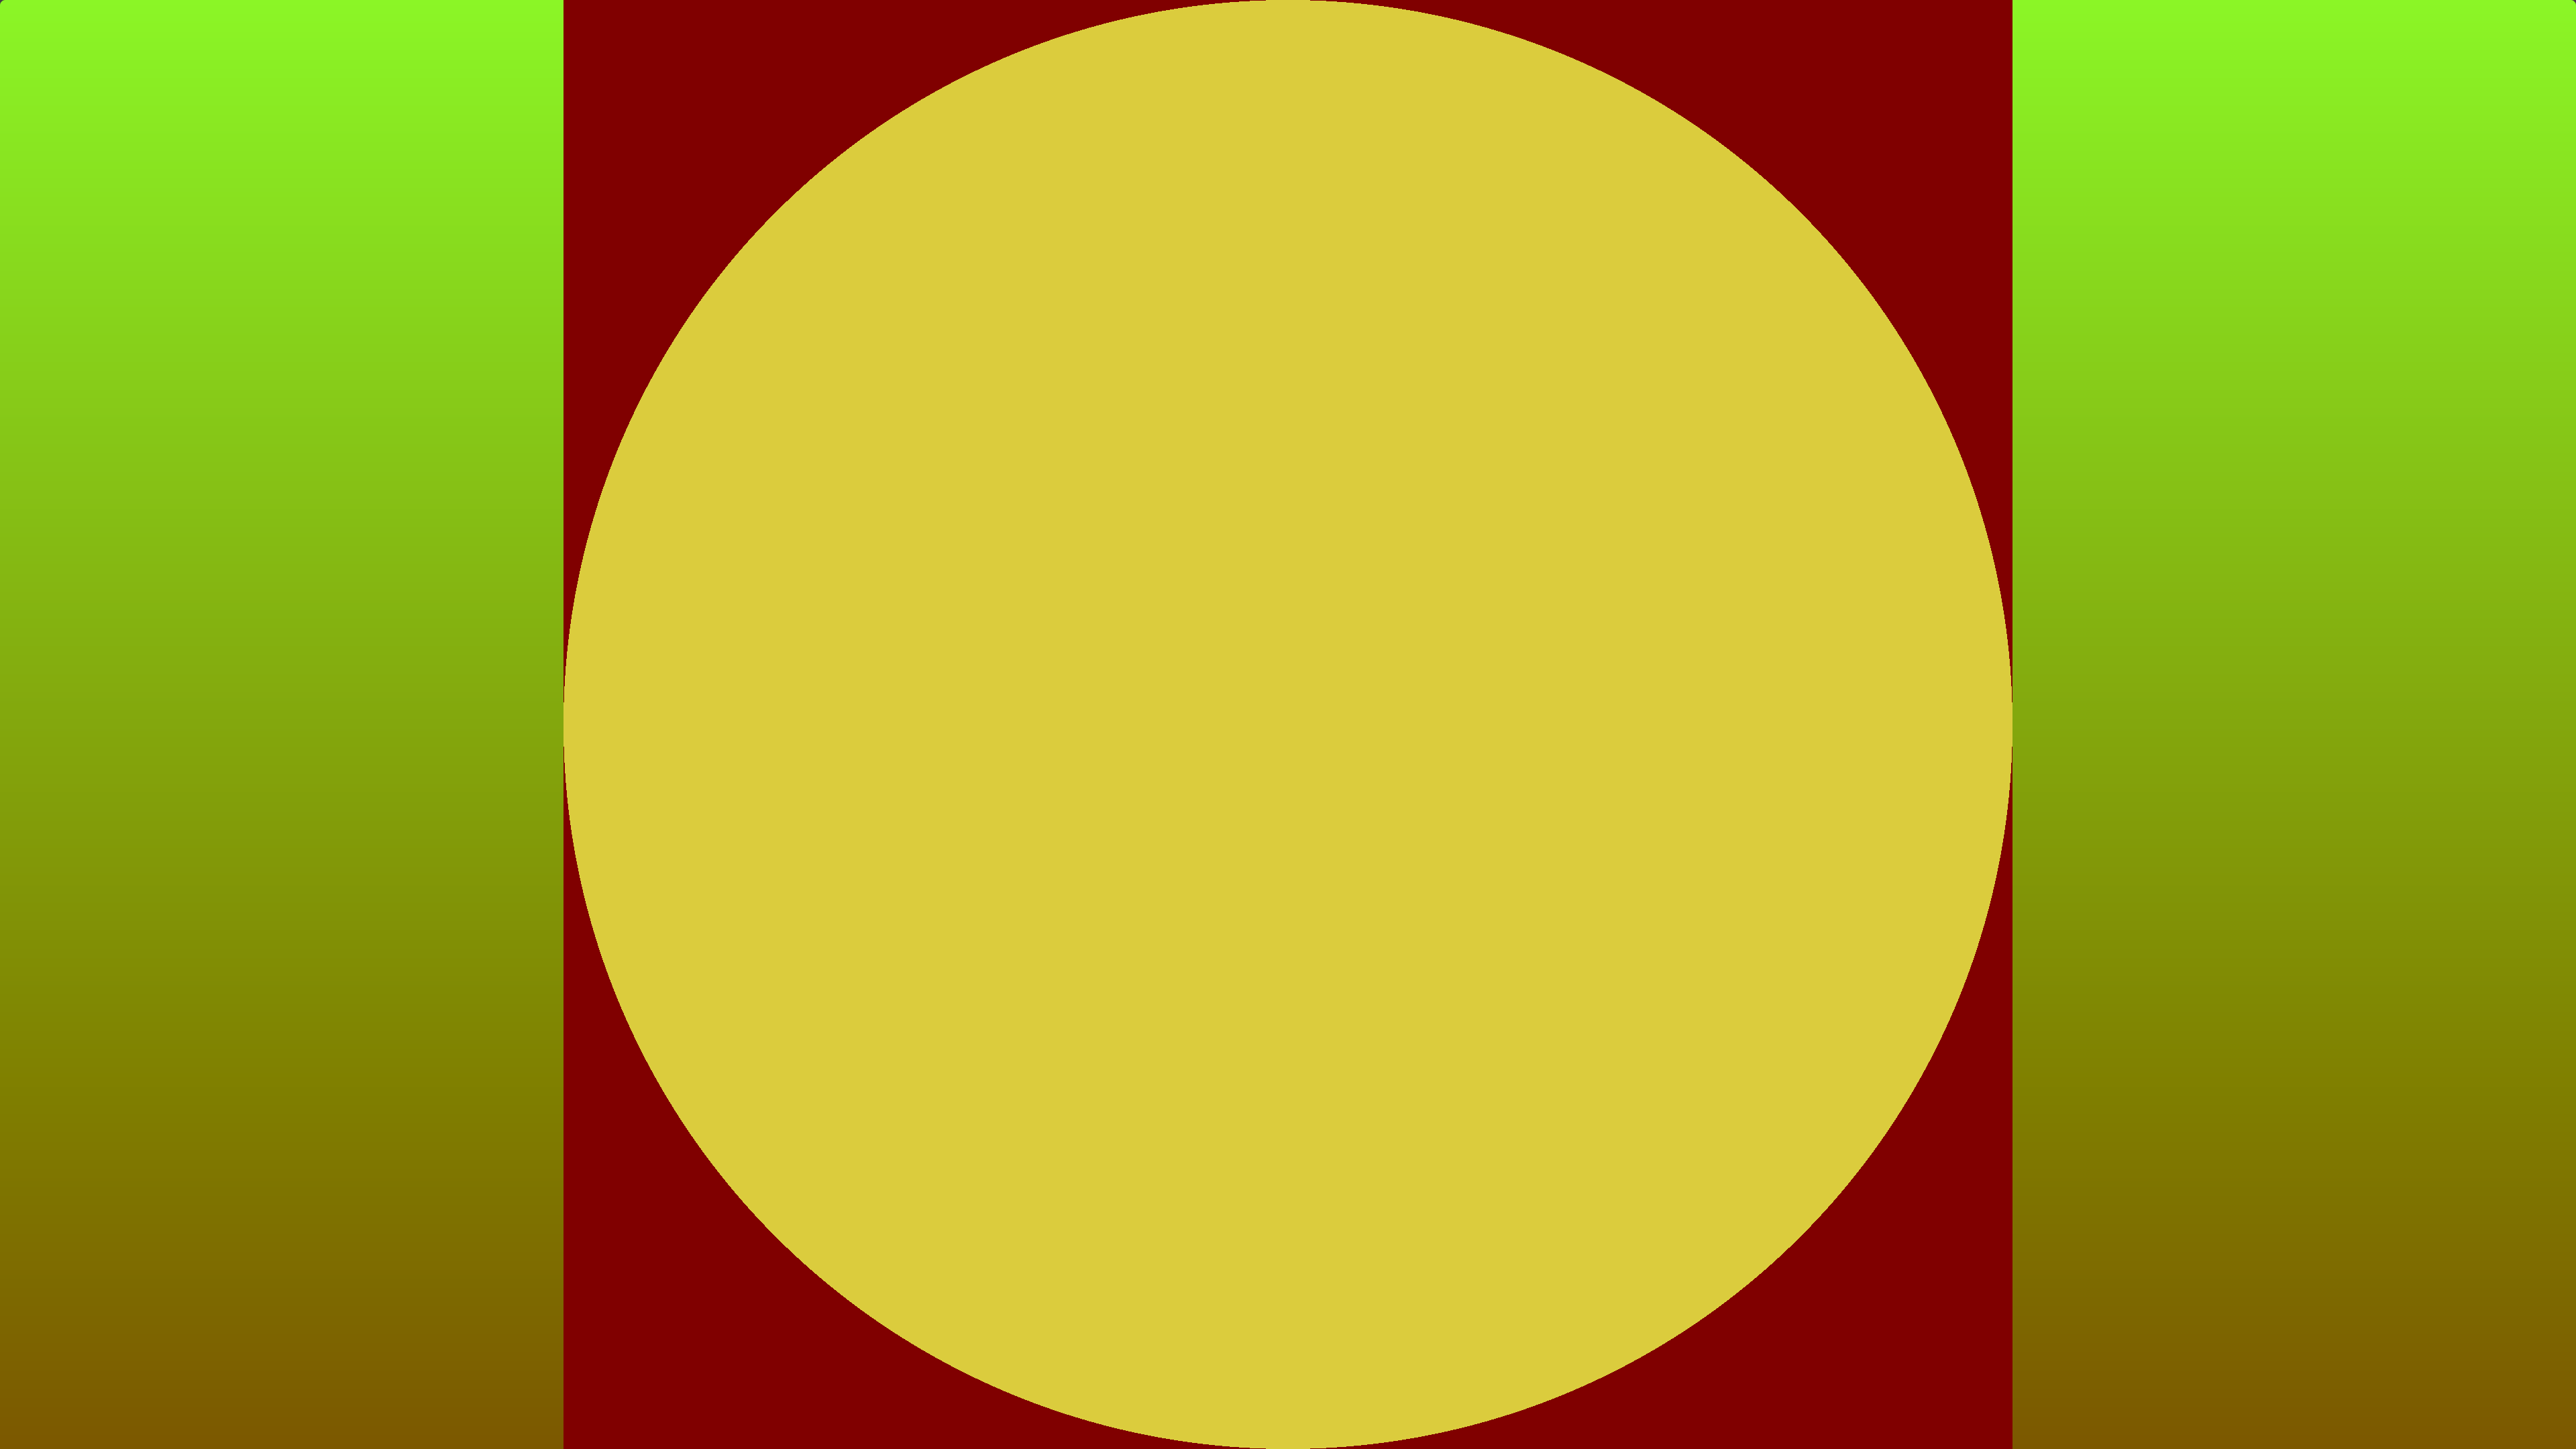
\includegraphics[width=0.6\textwidth]{img/Ejer2}
        \end{figure}
\end{columns}
\end{frame}

\begin{frame}{Transformaciones Afines}
Hay una definición formal de \href{https://en.wikipedia.org/wiki/Affine_transformation}{transformación afín}. Pero para nuestros propósitos, podremos decir que: una transformación afín $A: \mathbb{R}^n \rightarrow \mathbb{R}^n$ es una transformación lineal seguida de una traslación.

\begin{block}{}
    Si $\mathbf{x} \in \mathbb{R}^n$, $M$ es una matriz de $n \times n$ y $\mathbf{d} \in \mathbb{R}^n$ un vector.
    Entonces $A(\mathbf{x}) = M \mathbf{x} + \mathbf{d}$ es una transformación afín.
\end{block}
\begin{itemize}
    \item Todas las transformaciones lineales son transformaciones afines (con $\mathbf{d} = \mathbf{0}$)
    \item Todas las traslaciones son transformaciones afines (con $M = I$).
\end{itemize}
\end{frame}


\begin{frame}{Coordenadas homogéneas}

\begin{itemize}
    \item Todas las transformaciones lineales pueden llevarse a cabo multiplicando matrices.
    \item Pero las traslaciones no se pueden llevar a cabo multiplicando matrices
    \item Para solucionar ese problemas usamos las \href{https://en.wikipedia.org/wiki/Homogeneous_coordinates}{coordenadas homogéneas}
\end{itemize}
Vamos a adoptar la convención de que tanto puntos, como vectores son representados en columna.
\begin{block}{}
    Las coordenadas homogéneas de un punto $\mathbf{x} \in \mathbb{R}^n$, son una tupla de $n+1$ componentes, formada por los $n$ componentes de $\mathbf{x}$, seguidos por el escalar 1.
\end{block}
Ésta \emph{no es} la definición general, pero hará las explicaciones mas sencillas.
\begin{itemize}
    \item Las coordenadas homogéneas representan al punto $\mathbf{x} \in \mathbb{R}^n$ con un punto $\mathbf{x}_{h} \in \mathbb{R}^{n+1}$.
    \item Pero permiten \emph{expresar las transformaciones afines como una multiplicación de matrices}.
\end{itemize}

\end{frame}

\begin{frame}{Traslación}
\begin{columns}
\column[t]{0.5\textwidth}
\begin{itemize}
    \item Traslada una curva en el espacio
    \item Tiene parámetro el vector de traslación $\mathbf{t}$
    \item Se puede expresar con la siguiente matriz:
\end{itemize}
$$
\begin{pmatrix}
1 & 0 & t_x\\
0 & 1 & t_y\\
0 & 0 & 1
\end{pmatrix}
\begin{bmatrix}
x \\
y \\
1 \\
\end{bmatrix}
=
\begin{bmatrix}
x + t_x \\
y + t_y \\
1 \\
\end{bmatrix}
$$
\begin{itemize}
    \item Si $\mathbf{t} = \mathbf{0}$, hay una operación nula
    \item La operación inversa es trasladar por $-\mathbf{t}$
    \item La figura muestra una traslación por $\mathbf{t} = (2, 1)^t$
\end{itemize}
\column[t]{0.5\textwidth}
\begin{figure}[htp]
 \centering
 \begin{subfigure}[b]{0.4\textwidth}
   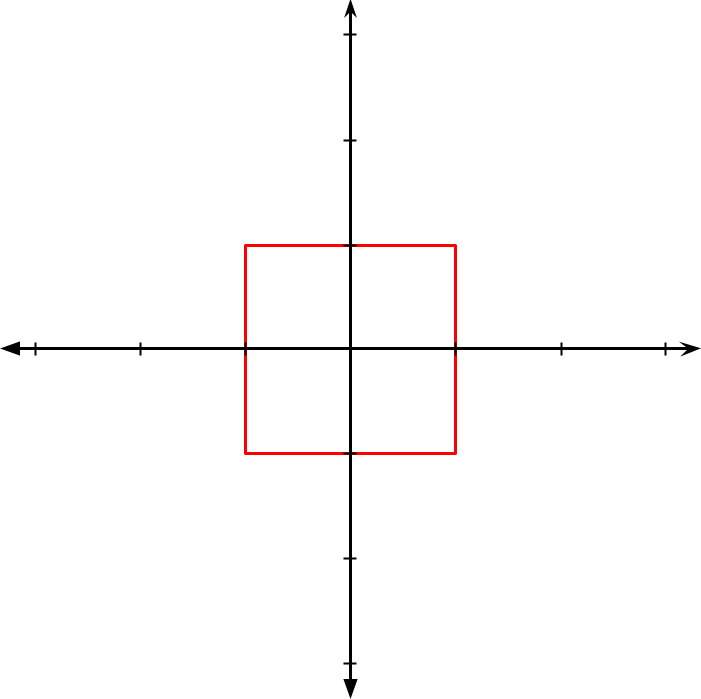
\includegraphics[width=\textwidth]{img/Square}
 \end{subfigure}
\\
\vspace{0.15cm}
 \begin{subfigure}[b]{0.4\textwidth}
   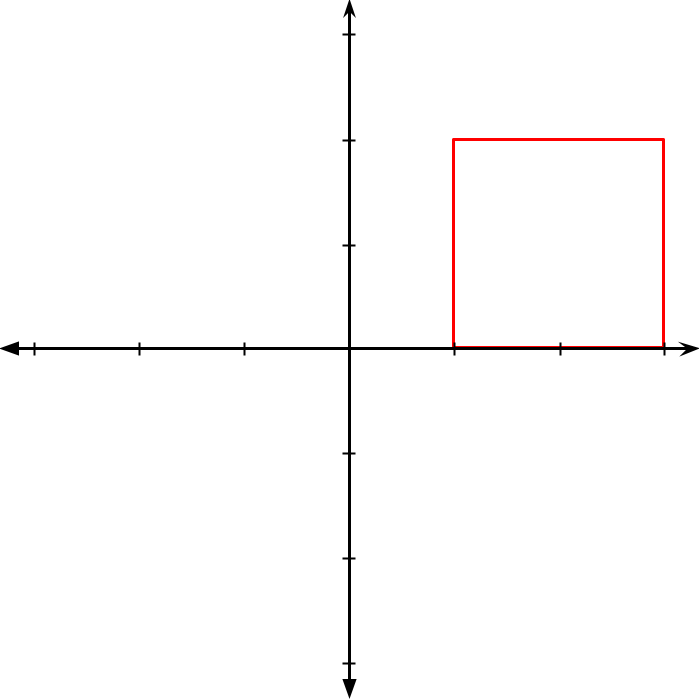
\includegraphics[width=\textwidth]{img/Translated}
 \end{subfigure}
\end{figure}
\end{columns}
\end{frame}

\begin{frame}{Rotación}
\begin{columns}
\column[t]{0.5\textwidth}
\begin{itemize}
    \item Rota una curva \emph{alrededor del origen}
    \item Tiene parámetro el angulo de rotación $\theta$
    \item Se puede expresar con la siguiente matriz:
\end{itemize}
$$
\begin{pmatrix}
\cos \theta & -\sin \theta & 0 \\
\sin \theta & \cos \theta & 0 \\
0 & 0 & 1
\end{pmatrix}
\begin{bmatrix}
x \\
y \\
1 \\
\end{bmatrix}
=
\begin{bmatrix}
x \cos \theta - y \sin \theta \\
x \sin \theta + y \cos \theta  \\
1 \\
\end{bmatrix}
$$
\begin{itemize}
    \item Si $\theta = 0$, hay una operación nula
    \item La operación inversa es rotar por $-\theta$
    \item La figura muestra una rotación de $\theta = \frac{\pi}{4}$
\end{itemize}
\column[t]{0.5\textwidth}
\begin{figure}[htp]
 \centering
 \begin{subfigure}[b]{0.4\textwidth}
   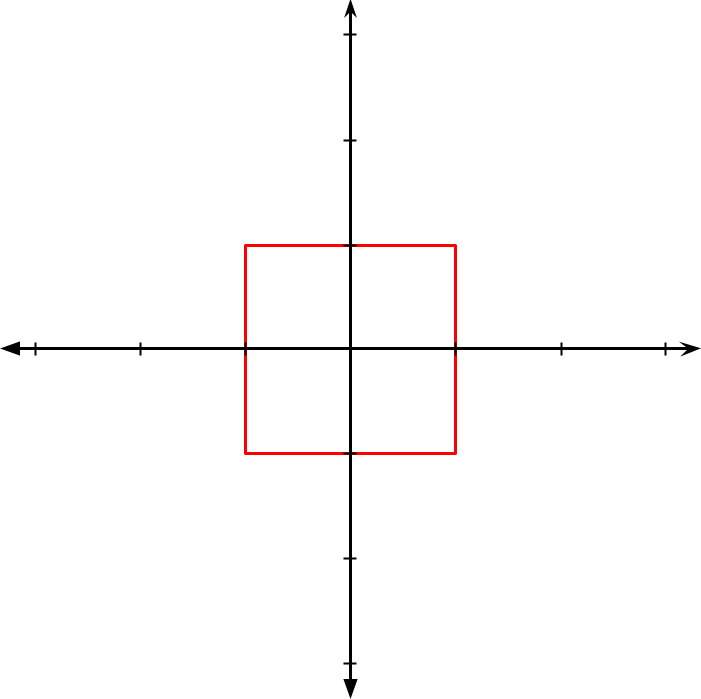
\includegraphics[width=\textwidth]{img/Square}
 \end{subfigure}
\\
\vspace{0.15cm}
 \begin{subfigure}[b]{0.4\textwidth}
   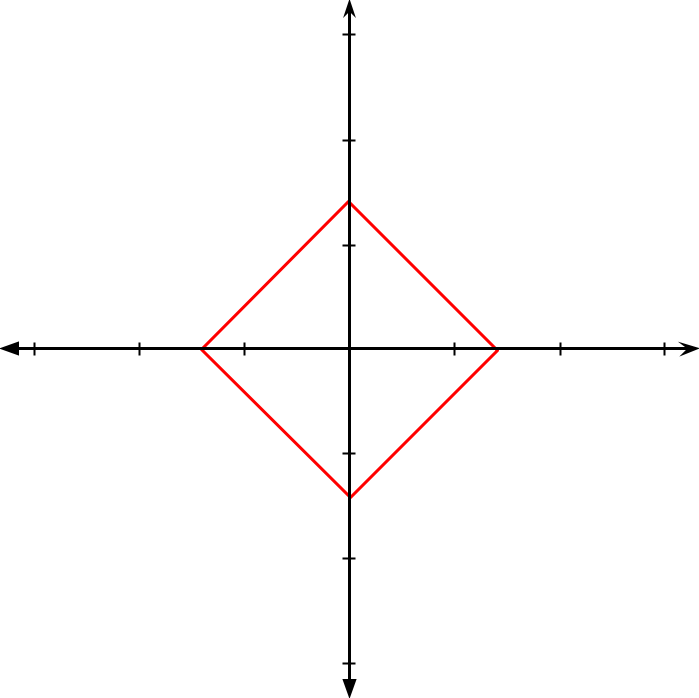
\includegraphics[width=\textwidth]{img/Rotated}
 \end{subfigure}
\end{figure}
\end{columns}
\end{frame}

\begin{frame}{Escalamiento}
\begin{columns}
\column[t]{0.5\textwidth}
\begin{itemize}
    \item Escala una curva \emph{con respecto al origen}
    \item Tiene parámetro el factor de escala $\mathbf{s}$
    \item Se puede expresar con la siguiente matriz:
\end{itemize}
$$
\begin{pmatrix}
s_x & 0 & 0 \\
0 & s_y & 0 \\
0 & 0 & 1
\end{pmatrix}
\begin{bmatrix}
x \\
y \\
1 \\
\end{bmatrix}
=
\begin{bmatrix}
s_x \cdot x  \\
s_y \cdot y  \\
1 \\
\end{bmatrix}
$$
\begin{itemize}
    \item Si $\mathbf{s} = ( 1 , 1 )^t$, hay una operación nula
    \item La operación inversa es escalar por $\mathbf{s} = (\frac{1}{s_x} , \frac{1}{s_y} )^t$
    \item La figura muestra un escalamiento por $\mathbf{s} = ( \frac{1}{2} , 2 )^t$
\end{itemize}
\column[t]{0.5\textwidth}
\begin{figure}[htp]
 \centering
 \begin{subfigure}[b]{0.4\textwidth}
   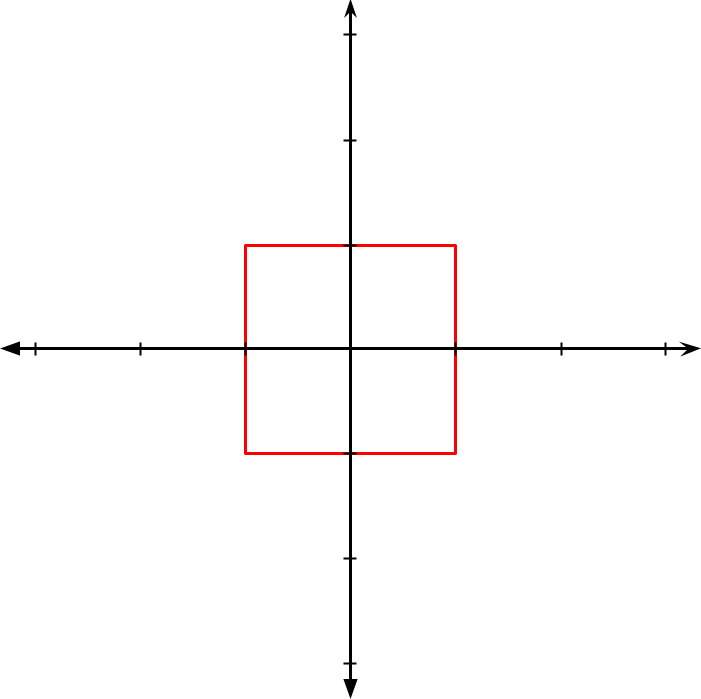
\includegraphics[width=\textwidth]{img/Square}
 \end{subfigure}
\\
\vspace{0.15cm}
 \begin{subfigure}[b]{0.4\textwidth}
   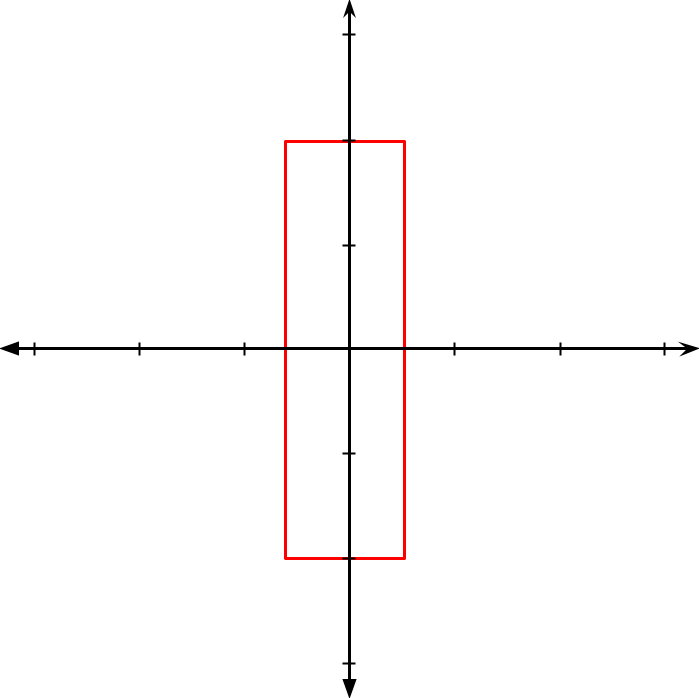
\includegraphics[width=\textwidth]{img/Scalated}
 \end{subfigure}
\end{figure}
\end{columns}
\end{frame}

\begin{frame}{Composición de transformaciones afines}
Las transformaciones afines, se pueden aplicar una después de otra. 
\begin{itemize}
    \item Esto se llama \alert{composición de transformaciones}
    \item Y es particularmente útil que se haga con matrices
    \item La multiplicación de matrices es asociativa 
    $$T_1 T_2 T_3 \mathbf{x} = T_1 (T_2 (T_3 \mathbf{x})) = (T_1 T_2 T_3) \mathbf{x}$$
    \item La multiplicación de matrices no es conmutativa: 
    $$T_1 T_2 \mathbf{x} \neq T_2 T_1 \mathbf{x}$$
\end{itemize}
\end{frame}

\begin{frame}{Ejemplo}
Si $R$ fuera una rotación de $\frac{5\pi}{4}$ y $S$ escalameinto por $(\frac{1}{2}, 2)^t$
\begin{figure}[htp]
 \centering
 \begin{subfigure}[b]{0.25\textwidth}
   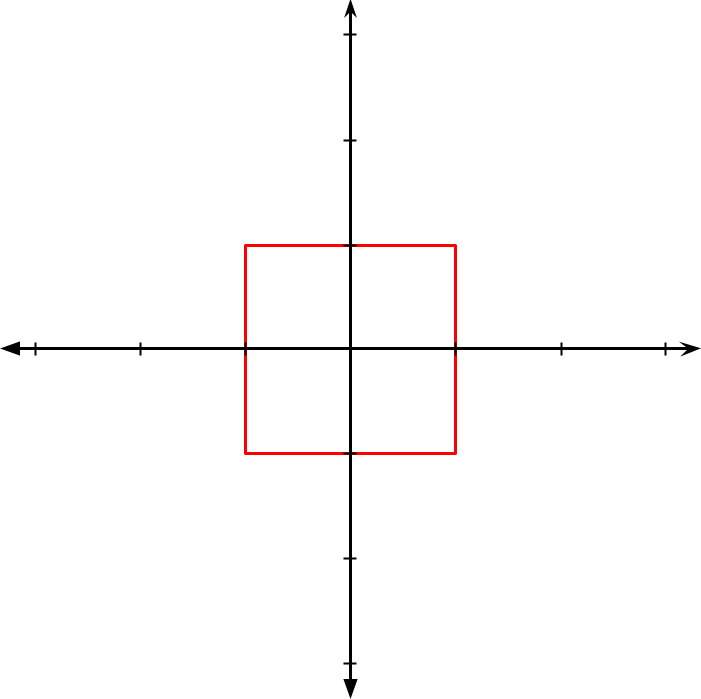
\includegraphics[width=\textwidth]{img/Square}
   \caption{Figura original}
 \end{subfigure}
 ~
 \begin{subfigure}[b]{0.25\textwidth}
   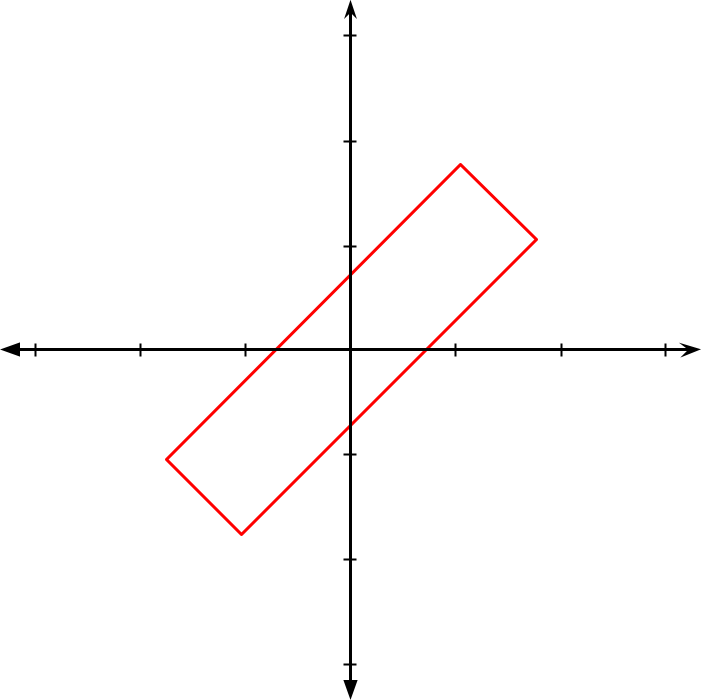
\includegraphics[width=\textwidth]{img/ScaleRoate}
   \caption{$R S \mathbf{x} = ( R ( S \mathbf{x}))$}
 \end{subfigure}
 ~
 \begin{subfigure}[b]{0.25\textwidth}
   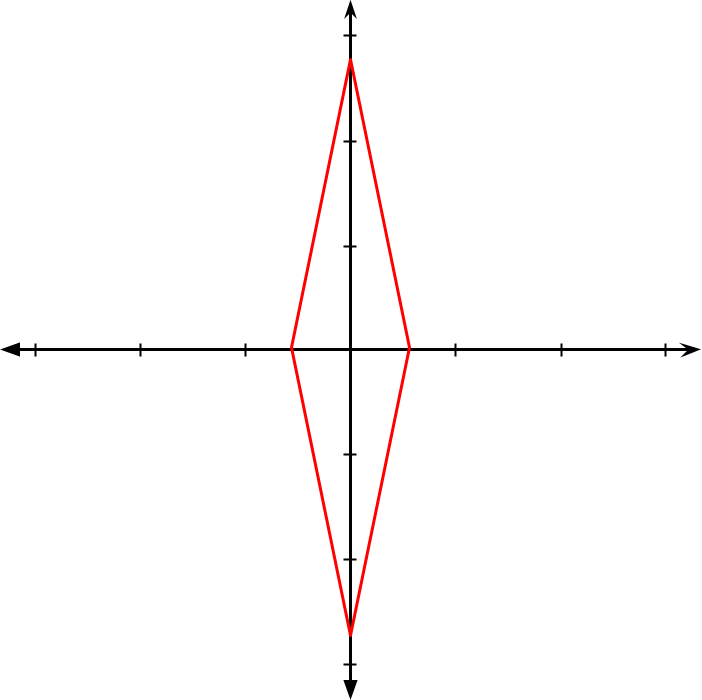
\includegraphics[width=\textwidth]{img/RoateScale}
   \caption{$S R \mathbf{x} = (S (R \mathbf{x}))$}
 \end{subfigure}
\end{figure}
\end{frame}

\begin{frame}{Transformaciones afines en Shadertoy}
\begin{itemize}
    \item La explicación anterior es como se hacen las gráficas tradicionalmente.
    \item Es decir, transformamos la geométrica para acomodarla en el espacio.
\end{itemize}
\begin{alertblock}{En Shadertoy en 2D hacemos lo contrario}
    \begin{itemize}
        \item En shadertoy en 2D, trasformamos las coordenadas del fragment hacia la figura.
        \item Esto es equivalente a decir que transformamos el espacio hacia la figura.
        \item Por lo tanto, para situar figuras en 2D usamos la matriz inversa de la matriz de trasformación.
    \end{itemize}
\end{alertblock}
\end{frame}

\begin{frame}[fragile]{Ejemplo en Shadertoy 2D}
\begin{listing}
\begin{minted}{glsl}
mat3 M = translate(vec2(0.75, 0.0)) * scale(vec2(0.25));

float disCircle = sdfCircle(inverse(M) * coord);

color = mix(Red, color, step(0.0, disCircle));
\end{minted}
\end{listing}
\begin{itemize}
    \item En este ejemplo se escala y luego se traslada una figura (circulo)
    \item Nótese la inversión de la matriz, antes de evaluar las sdf.
    \item Y el uso de la función \mintinline{glsl}{step} dentro de la función \mintinline{glsl}{mix}, para cambiar el color del fragment si estaba dentro de la figura.
\end{itemize}
\end{frame}

\begin{frame}{Ejercicio: Figuras animadas}
\url{https://github.com/nemediano/tallerShadertoy/tree/main/codigo/Ejercicio3}
\begin{columns}
\column[t]{0.5\textwidth}
     \begin{itemize}
         \item Usar transformaciones compuestas para crear una escena
         \item Puedes utilizar la \href{https://iquilezles.org/articles/distfunctions2d/}{esta lista} para ver mas figuras
         \item Puedes comenzar con el código del ejercicio anterior 
     \end{itemize}
\column[t]{0.5\textwidth}
        \begin{figure}[htb]
            \centering
            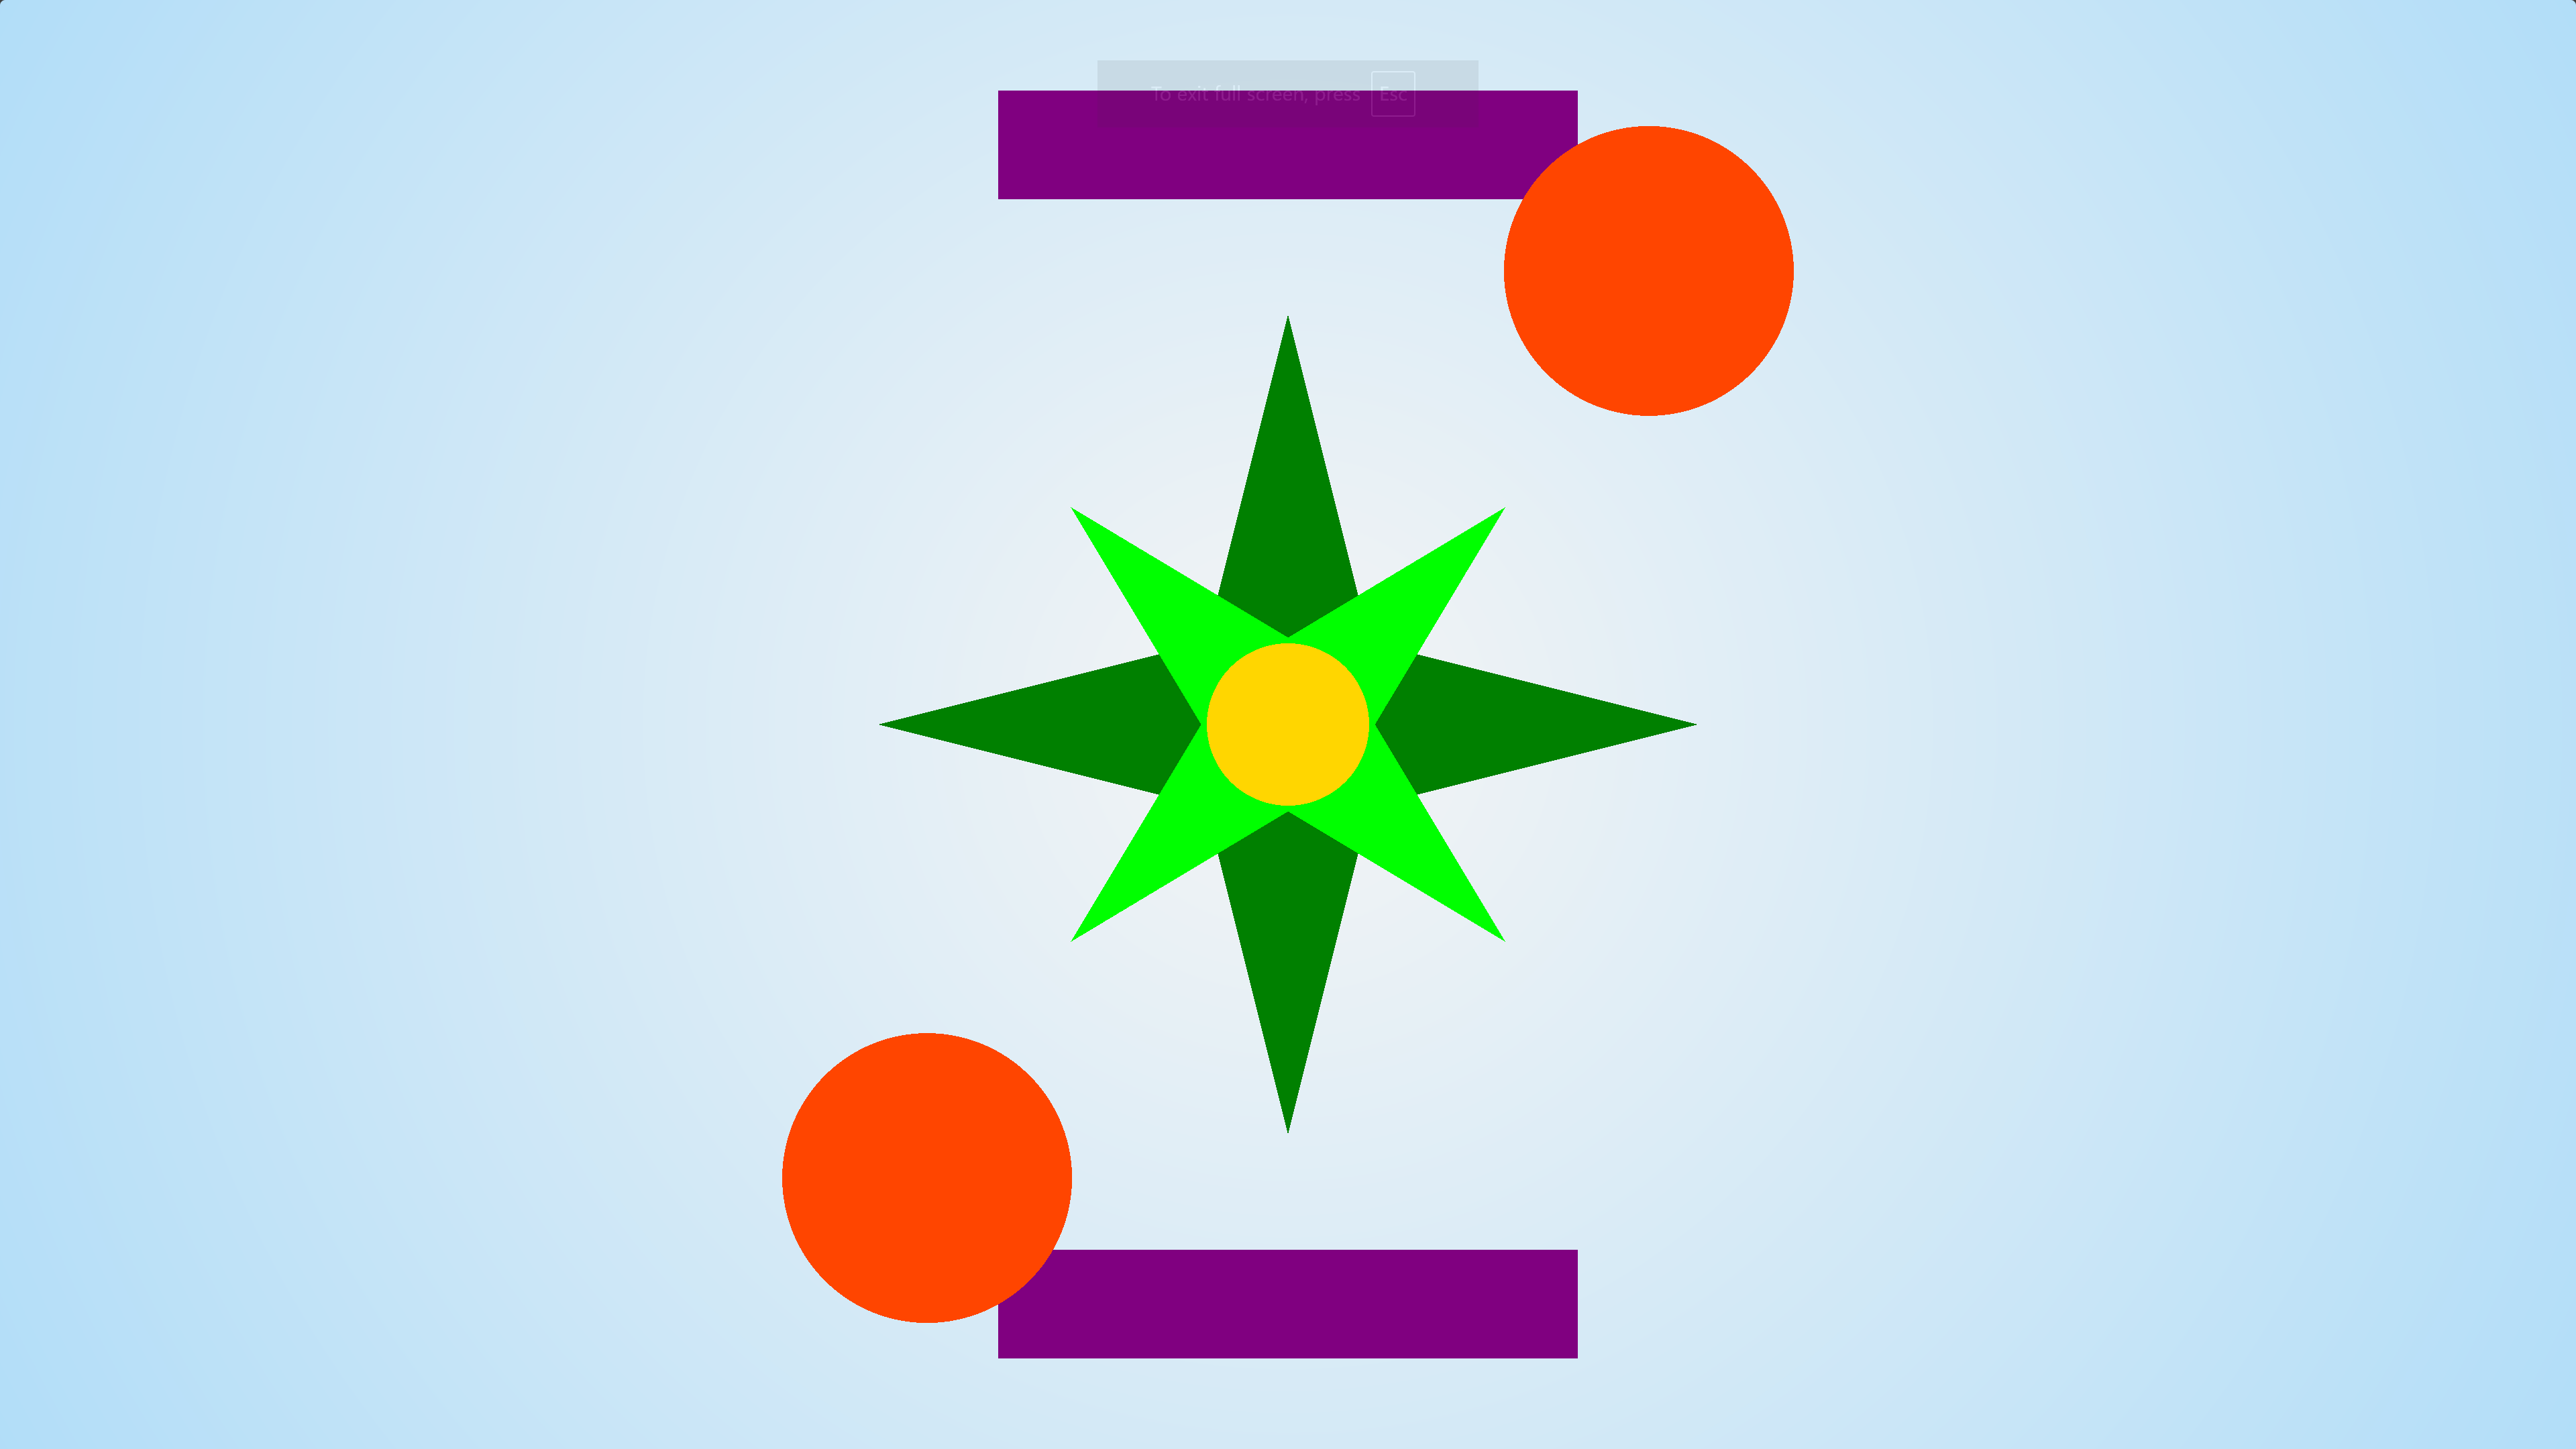
\includegraphics[width=0.6\textwidth]{img/Ejer3}
        \end{figure}
\end{columns}
\end{frame}
